\documentclass[tikz,border=6pt]{standalone}
\usepackage[T1]{fontenc}
\usetikzlibrary{calc}
\begin{document}
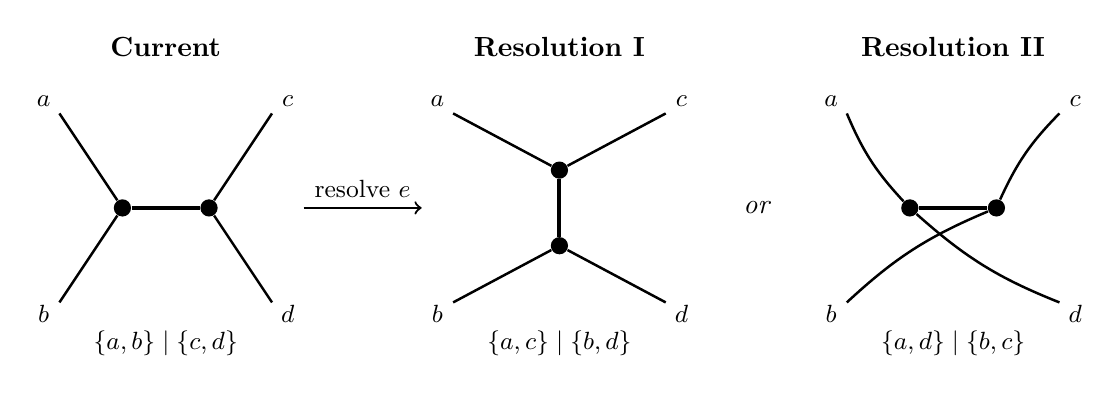
\begin{tikzpicture}[
  vertex/.style={circle,fill=black,inner sep=2.2pt},
  leg/.style={line width=0.9pt},
  middle/.style={line width=1.4pt},
  every node/.style={font=\small}
]
  \foreach \x/\heading in {0/Current,5/Resolution I,10/Resolution II}{
    \node[font=\bfseries] at (\x,2.05) {\heading};
    \coordinate (nw) at (\x-1.35,1.2);
    \coordinate (sw) at (\x-1.35,-1.2);
    \coordinate (ne) at (\x+1.35,1.2);
    \coordinate (se) at (\x+1.35,-1.2);
    \node at ($(nw)+(-.2,.15)$) {$a$};
    \node at ($(sw)+(-.2,-.15)$) {$b$};
    \node at ($(ne)+(.2,.15)$) {$c$};
    \node at ($(se)+(.2,-.15)$) {$d$};
  }

  % Current partition {a,b}|{c,d}.
  \node[vertex] (u0) at (-.55,0) {};
  \node[vertex] (v0) at (.55,0) {};
  \draw[middle] (u0)--(v0);
  \draw[leg] (-1.35,1.2)--(u0) (-1.35,-1.2)--(u0);
  \draw[leg] (1.35,1.2)--(v0) (1.35,-1.2)--(v0);
  \node at (0,-1.72) {$\{a,b\}\mid\{c,d\}$};

  % Resolution I: {a,c}|{b,d}.
  \node[vertex] (u1) at (5,.48) {};
  \node[vertex] (v1) at (5,-.48) {};
  \draw[middle] (u1)--(v1);
  \draw[leg] (3.65,1.2)--(u1) (6.35,1.2)--(u1);
  \draw[leg] (3.65,-1.2)--(v1) (6.35,-1.2)--(v1);
  \node at (5,-1.72) {$\{a,c\}\mid\{b,d\}$};

  % Resolution II: {a,d}|{b,c}.
  \node[vertex] (u2) at (9.45,0) {};
  \node[vertex] (v2) at (10.55,0) {};
  \draw[middle] (u2)--(v2);
  \draw[leg] (8.65,1.2) to[bend right=10] (u2);
  \draw[leg] (11.35,-1.2) to[bend left=10] (u2);
  \draw[leg] (8.65,-1.2) to[bend left=10] (v2);
  \draw[leg] (11.35,1.2) to[bend right=10] (v2);
  \node at (10,-1.72) {$\{a,d\}\mid\{b,c\}$};

  \draw[->,line width=.8pt] (1.75,0)--(3.25,0)
    node[midway,above] {resolve $e$};
  \node[font=\itshape] at (7.5,0) {or};
\end{tikzpicture}
\end{document}
